% https://trac.ffmpeg.org/wiki

\title{\href{http://www.milkytracker.org/}{MilkyTracker}}

\maketitle
\tableofcontents

\section{What is MilkyTracker?}

\begin{itemize}
\item MilkyTracker a sound tracker (in other words, a music
  sequencer). It represents music tracks as an arrangement of discrete
  musical notes positioned in one of several channels, at discrete
  chronological positions on a timeline.
\end{itemize}

\begin{center}
  %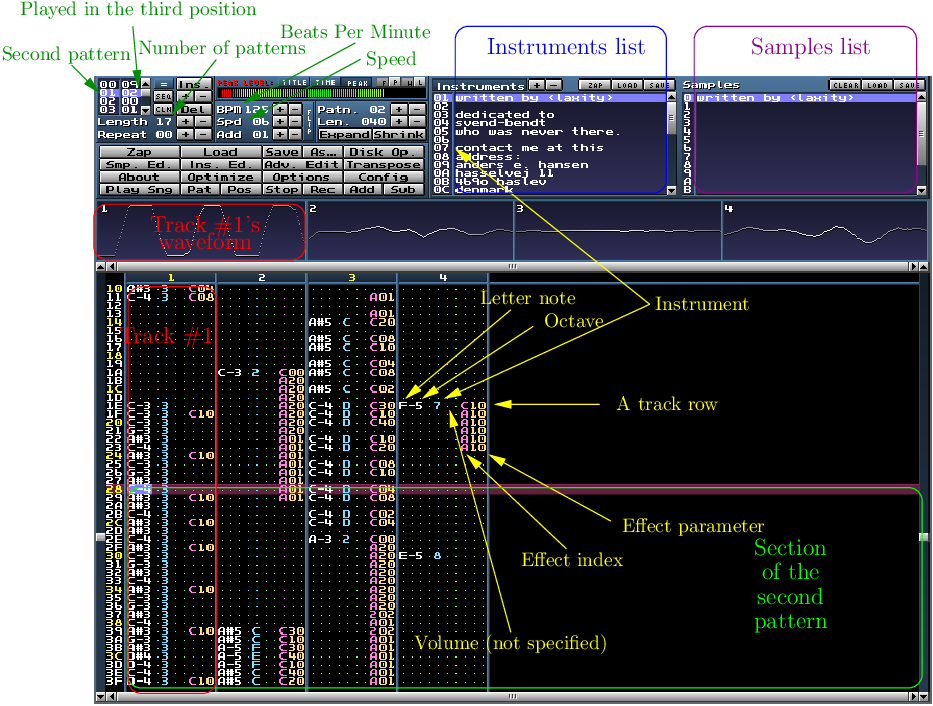
\includegraphics{milky-tracker-description.png}
\end{center}

\section{A little bit of history about trackers}

\begin{itemize}
\item Sound trackers were born with the
  \href{http://en.wikipedia.org/wiki/Amiga}{Commodore Amiga} in
  1985. The Amiga mounted an audio coprocessor named
  \href{http://en.wikipedia.org/wiki/Original_Chip_Set}{Paula}, which
  could be ``programmed'' by sending a \emph{module} through
  \href{http://en.wikipedia.org/wiki/Direct_memory_access}{DMA}
  producing something similar to
  \href{http://en.wikipedia.org/wiki/Wavetable_synthesis}{wavetable
    mixing}. Paula can mix up to 4 sequences (tracks) of signed
  linear-quantized 8-bit two's complement PCM sound samples and send
  the mixed sound to an stereo
  \href{http://en.wikipedia.org/wiki/Digital-to-analog_converter}{DAC}.

\item In 1987, the sound arrives shyly to the PC with the
  \href{http://en.wikipedia.org/wiki/Sound_Blaster}{Sound
    Blaster}. This year
  \href{http://woolyss.com/tracking-trackers.php?s=Amiga}{the
    first\footnote{Published and that has survived until the time
      being.} amiga module},
  \href{http://modarchive.org/index.php?request=view_by_moduleid&query=33438}{amegas},is
  created by Karsten Obarski, the creator of the first module tracker
  \href{http://en.wikipedia.org/wiki/Ultimate_Soundtracker}{The
    Ultimate SoundTracker}.

\item In 1989, there are thousands of modules, such as
  \href{http://modarchive.org/index.php?request=view_by_moduleid&query=97751}{electricity}.

\item During the 1990s, tracker musicians gravitated from Amiga
  platforms to the PC, which started to mount sound cards such as the
  \href{http://en.wikipedia.org/wiki/Sound_Blaster_16}{Sound Blaster
    16} and
  \href{http://en.wikipedia.org/wiki/Gravis_Ultrasound}{Gravis
    Ultrasound (GUS)}. For example, GUS cards can mix up to 32
  channels of CD Quality (44.1 kHz/16 bit/Stereo).

\item In the following years, as CPUs got faster and acquired special
  multimedia processing abilities (e.g.
  \href{http://en.wikipedia.org/wiki/MMX\_\%28instruction_set\%29}{MMX}),
  the responsibility for audio mixing passed from hardware to
  software, which gradually enabled the use of more and more channels
  (the ``record'' belong to
  \href{http://en.wikipedia.org/wiki/Impulse_Tracker}{Impulse Tracker}
  which can handle up to 64 channels).

\item MilkyTracker was created in mid-90s to emulate the popular
  \href{http://en.wikipedia.org/wiki/FastTracker_2}{Fasttracker II}
  DOS and the Amiga
  \href{http://sourceforge.net/projects/protracker/}{ProTracker 2/3} 
  programs.

\item In 1998, amazing pieces such as
  \href{http://modarchive.org/index.php?request=view_by_moduleid\&query=58684}{squired}
  have being created.

\item Still some musicians use this format to create their
  compositions. An example:
  \href{http://modarchive.org/index.php?request=view_by_moduleid\&query=173932}{Pinochet
    Asesino}.

\end{itemize}

\section{What is a music module?}
\begin{itemize}
\item Basically, a
  \href{http://en.wikipedia.org/wiki/MOD\_\%28file_format\%29}{module}
  is a collection of tracks which store samples, notes, volumes and
  effects, indicating how and when the samples are to be played. More
  accurately,
  \href{http://www.wildbunny.co.uk/blog/2012/05/15/composing-in-game-music/}{Music
    modules} are a hybrid between the sequenced type of music files
  like MIDI and wave files. Like MIDI files, modules contain
  specifications about what instrument to play, at which pitch, using
  which effects, and so on. However, they also include the actual
  samples to play.

\item The samples are usually short in time, one shot sounds (like
  bass drums, snares) or samples (in fact, sequences of audio samples)
  that are can be looped to emulate a sustaining note (like strings,
  leads). 

%\item Best to Worst Module files: IT > MO3 > XM > S3M > MED > MOD

\end{itemize}

\section{How can I play a module in Linux?}
Some options:
\begin{enumerate}

\item \href{http://sourceforge.net/projects/xmp/}{xmp}: xmp is a
  module player for Unix-like systems that plays over 90 mainstream
  and obscure module formats from Amiga, Atari, Acorn, Apple IIgs and
  PC, including Protracker (MOD), Scream Tracker 3 (S3M), Fast Tracker
  II (XM) and Impulse Tracker (IT) files.

\item \href{http://www.cubic.org/player/}{Open Cubic Player (ocp)}: a
  audio player with several interface capabilities.

\item \href{http://en.wikipedia.org/wiki/VLC_media_player}{VLC}: of
  course, why not?

\item \href{http://en.wikipedia.org/wiki/XMMS}{XMMS}: a Winamp clone.

\item
  \href{http://en.wikipedia.org/wiki/Audacious\_\%28software\%29}{Audacious:}
  An excelent audio player with a Jack interface.

\end{enumerate}

\section{Some more definitions}
\begin{itemize}

\item \href{http://en.wikipedia.org/wiki/Music_tracker}{Pattern}: A
  pattern is a group of simultaneously played tracks that represents a
  full section of the song. Patters have a fixed number of rows
  (typically 64) on which notes and effects can be placed (most
  trackers lay out tracks in a vertical fashion) and may be repeated
  throughout a song.

\item \href{http://en.wikipedia.org/wiki/Music_tracker}{Order}: An
  order is part of any sequence of patterns which defines the layout of
  a song. Patterns can be repeated across multiple orders to save
  tracking time and file space.

\item
  \href{http://www.linuxplanet.com/linuxplanet/tutorials/4363/1}{Track}:
  The section of a pattern which is sequenced in an independent DAC
  channel, providing thus
  \href{http://en.wikipedia.org/wiki/Polyphony}{poliphony}\footnote{For
    example, A basic drum set could thus be arranged by putting a bass
    drum at rows 0, 4, 8, 12 etc. of one track and putting some hihat
    at rows 2, 6, 10, 14 etc. of a second track. Of course bass and
    hats could be interleaved on the same track, if the samples are
    short enough. If not, the previous sample is usually stopped when
    the next one begins. Some
    \href{http://en.wikipedia.org/wiki/Music_tracker}{modern trackers
      simulate polyphony} in a single track by setting the "new note
    action" of each instrument to cut, continue, fade out, or release,
    opening new mixing channels as necessary. Without poliphony, the
    number of notes that can be played simultaneously depends on how
    many "tracks" there are per pattern.}. Tracks are like individual
  members of an orchestra, except that your orchestra consists of
  little chunks of music rather (samples) than specific
  instruments. Whereas the original Amiga trackers only provided four
  tracks due to the hardware limits, modern trackers can mix a
  virtually unlimited number of channels into one sound stream through
  software mixing.

\item \href{http://en.wikipedia.org/wiki/Music_tracker}{Tracking}: The
  process of composing module files.

\item
  \href{http://en.wikipedia.org/wiki/Ultimate_Soundtracker}{Channel}:
  Channel and track are synonymous. For example, MilkyTracker can mix
  up to 32 channels, meaning 32 sounds can play simultaneously.

\item
  \href{http://en.wikipedia.org/wiki/Musical_instrument}{Instrument}:
  A collection of one or more samples. Instruments are usually
  classified into four categories:
  \href{http://en.wikipedia.org/wiki/Rhythm_section#Instruments}{rhythm}
  (such as a bass drum),
  \href{http://en.wikipedia.org/wiki/Bass\_\%28instrument\%29}{bass}
  (such as a bass guitar),
  \href{http://www.howmusicworks.org/300/Chords-and-Harmony}{chords}
  (such as a guitar) and leads (such as a piano). An instrument is a
  single sample along with an optional indication of which portion of
  the sample can be repeated to hold a sustained note.

\item
  \href{http://dem0lecule.newgrounds.com/news/post/753500}{Instrument
    Editor}. Usually, when a new instrument is created, a sample is
  liked to it. In most trackers there is a panel to edit/add envelop,
  control the global volume, fading, panning, etc.

\item \href{http://en.wikipedia.org/wiki/Module_file}{Sample}: A
  sample is a small digital sound file of an instrument, voice, or
  other kind of sound. When very short samples are used (in order to
  reduce as much as possible the size of the module file), the module
  usually is called a
  \href{http://en.wikipedia.org/wiki/Chiptune}{chip tune} and
  \href{http://woolyss.com/chipmusic.php}{chip music} is produced.

\item \href{http://dem0lecule.newgrounds.com/news/post/753500}{Sample
    Editor}. It is very similar to Instrument Editor. This is where
  you put your audio file such as WAV.

\item \href{http://en.wikipedia.org/wiki/Note}{Note}: A note
  designates the frequency at which the sample is played back. By
  increasing or decreasing the playback speed of a digital sample, the
  pitch is raised or lowered, simulating instrumental notes (e.g. C,
  C\#, D, etc.).

\item \href{http://en.wikipedia.org/wiki/Tempo}{Tempo}: Controls the
  speed of the playback and usually is measured in BPM (Beats Per
  Minute).

\item
  \href{http://www.milkytracker.org/docs/MilkyTracker.html#effects}{Effect}:
  An effect is a special function applied to a particular note. Common
  tracker effects include volume, portamento, vibrato, retrigger,
  tremolo and arpeggio.

\item \href{http://en.wikipedia.org/wiki/Loudness}{Volume}: The energy
  of the note.

\item \href{http://en.wikipedia.org/wiki/Portamento}{Portamento}:
  Pitch sliding from one note to another.

\item \href{http://en.wikipedia.org/wiki/Vibrato}{Vibrato}: Regular
  and pulsating change of pitch of a note.

\item \href{http://en.wikipedia.org/wiki/Retrigger}{Retrigger}: When a
  sample is replayed a set number of times within a certain timeframe.

\item \href{http://en.wikipedia.org/wiki/Tremolo}{Tremolo}: The
  endure of a note produced either by rapid reiteration of a
  note, by rapid repeated slight variation in the pitch of a note, or
  by sounding two notes of slightly different pitches to produce
  prominent overtones.

\item \href{http://en.wikipedia.org/wiki/Arpeggio}{Arpegio}: When
  notes in a chord are played or sung in sequence, one after the
  other, rather than ringing out simultaneously.

\item
  \href{http://resources.openmpt.org/tracker_handbook/page/Glossary.htm}{Panning}:
  Is the control of the balance of a stereo or multichannel signal.

\item
  \href{http://milkytracker.org/docs/Vhiiula-TechniquesOfChipping.txt}{Echo}:
  Is the recursive playback of a sound slightly delayed and usually
  attenuated.

\item
  \href{http://en.wikipedia.org/wiki/Fade\_\%28audio\_engineering\%29}{Fading}:
  A gradual increase or decrease in the level of the sample.

\end{itemize}

\section{Getting samples}
\begin{itemize}
\item There are several alternatives:
  \begin{enumerate}
  \item \textbf{Recording}: You can create your own samples by playing
    an instrument like a guitar or a piano and recording (sampling)
    it.
  \item \textbf{Copying}: You could also extract sample sounds from a
    keyboard or a synthesizer, o even better, download them from
    Internet sites such as \url{http://freewavesamples.com/}.
  \item \textbf{Generating samples}: Another way to get samples is to
    generate them using a tool. This is actually done a lot for chip
    tunes because you can make some very small samples using this
    technique. Milky Tracker has some great options to facilitate
    this. For example, you can use basic shapes wave shapes as
    samples, or alter them by using the Draw function of Milky
    Tracker. It’s also possible to draw a sample from scratch.
  \end{enumerate}
\end{itemize}

\section{Getting sound modules}
\begin{itemize}
\item Many websites host large numbers of these files:
  \begin{enumerate}
  \item \href{http://modarchive.org/index.php}{The Mod Archive}: The
    most comprehensive.
  \item \href{ExoticA}{http://www.exotica.org.uk/wiki/Main\_Page}: An
    Amiga and retro gaming/computer music interest wiki including
    search-able computer music collections, game and demo scene
    information.
  \item \href{http://demodulate.scene.org/}{Demodulate}: are sites
    with demos and module music.
  \item \href{http://www.chiptune.com/}{Chiptune}\footnote{Clink on
      the error message to run the JavaScript Amiga Workbench!!}: An
    online community in respect and relation to chip music, art and
    its parallels.
  \item \href{http://www.mirsoft.info/gamemods.php}{WORLD OF GAME
      MODS}: A collection of game music modules for all platforms.
  \item \href{http://amp.dascene.net/home.php}{Amiga Music
      Preservation (AMP)}: A database about amiga music.
  \item \href{http://www.ankman.de/amiga-mod-music/}{Ankman's Amiga
      MOD music download page}: Pop, Techno, Dance, Trance and Game
    Music made with MOD trackers or the Amiga computer.
  \item \href{http://aminet.net/tree?path=mods}{Aminet}: Another
    module repository.
  \item \href{http://fby.develer.com/fby/modulescollection.html}{FBY
      MODULE COLLECTION}: A small FTP repository.
  \item \href{https://www.scenemusic.net/demovibes/}{Nectarine
      Demoscene Radio}: Not downloads avaiable. A live module-based
    radio operated by request of the registered users. Use, for example
\begin{verbatim}
vlc http://nectarine.from-de.com/necta192
\end{verbatim}
    to play it (however, notice that the stream in MP3, not a
    module!).
  \item \href{http://www.mazemod.org/}{Mazemod Radio}: A web radio
    dedicated to Amiga \& tracker music culture streaming various
    styles of computer electronic music from the demoscene \& computer
    art subculture.
  %\item \href{http://mods.abime.net/}{abime.net}: Another module-based
    %radio.
  \end{enumerate}
\end{itemize}

\section{Taxonomy of a track row (revisited)}
\begin{itemize}
\item Letter Note - Octave - Instrument (or Sample if no Instrument) -
  Volume - Effect Name - Effect Number.
\end{itemize}

\section{About keyboards}
\begin{itemize}
\item Most trackers support MIDI keyboards that allow to enter notes
  and volumes, easily.
\item Most trackers provide a graphical facility with a keyboard that
  can be controlled with the mouse.
\item Finally, most trackers maps the notes as follows: Q, A and Z is
  C note; W, S \& X is C\#, and so on.
\end{itemize}

\section{Effects (FX)}
\begin{itemize}
\item See
  \href{http://www.milkytracker.org/docs/MilkyTracker.html\#commands}{The
    Milky Tracker Manual}.
\end{itemize}

\section{Please, no more theory!!!}
\begin{enumerate}
\item Load an instrument from \url{http://freewavesamples.com/}.
\item Enter using only one channel (track):
\begin{verbatim}
BB = Beat
NN = Note
O  = Octave
II = Instrument
VV = Volume
E  = Effect index
ee = Effect parameter control

BB NNOIIVVEee
-- ----------
00 E-4.1..D00
 :          :
(the rest doesn't matter)

00 A-4.......
01 E-4.......
02 B-4.......
03 E-4.......
04 G-4.......
05 A-4.......
06 E-4.......
07 C-5.......
08 E-4.......
09 D-5.......
0A E-4.......
0B B-4.......
0C C-5.......
0D E-4.......
0E A-4.......
0F E-4.......
10 B-4.......
11 E-4.......
12 G-4.......
13 A-4.......
14 E-4.......
15 C-5.......
16 E-4.......
17 D-5.......
18 E-4.......
19 B-4.......
1A C-5.......
1B E-4.......
1C B-4....D00
 :          :
(the rest doesn't matter)
\end{verbatim}

\item Play it.

\item Now enter the same patters but using four channels (each row in
  a different track, cyclically). Do you think that using only one
  track, Milky Tracker provides poliphony?

\end{enumerate}

